\section{Research Methodology}
This chapter provides a detailed exposition of the methodology used throughout this work. This study has conducted exploratory and descriptive research to determine whether the use of simulation and an automated feedback driven system, a user can be trained as a race driver. The chapter is structured as follows: \S~\ref{sec:meth-overview} provides a general overview of the overarching methodology used in the study, \S~\ref{sec:meth-experiment-setup} describes in length the design of the instrument used to acquire experiment data and results, \S~\ref{sec:meth-experiment-structure} presents the experimental procedure and the rationale behind it, \S~\ref{sec:meth-data-gathering} identifies the information and data acquired through the experimental and descriptive methodologies employed, and finally \S~\ref{sec:meth-data-analysis} presents the data analysis mechanisms employed to substantiate our conclusions.
%
% Overview
%
\subsection{Overview}
\label{sec:meth-overview}
This study conducted experimental and descriptive research on the viability of the use of simulators in conjunction with an automated feedback system for improving race driving skills in the normal population. Specifically, a user study was devised and carried out with the primary goals being:
\begin{enumerate}
	\item To determine whether a context-based feedback system can improve the skills of a participant
	\item To quantify the magnitude of this improvement, if (1) is true
\end{enumerate}

These goals were addressed by means of an experimental setup based on a race-driving simulator, using which objective measurement of the participant performance could be gathered and analysed, and a questionnaire for relating the participant's experience with the experimentally-gathered data. The setup of the experiment is explored in more detail in \S~\ref{sec:meth-experiment-setup}.

Since the main goal of this study is that of assessing how effective a feedback system is in the learning process, the independent variable in the experiment is the ability to receive feedback. The hypothesis is that participant performance (such as average lap time) is improved through feedback, and is thus a dependent variable. However, practising without feedback can also lead to changes in the dependent variable; therefore this is controlled for by having two groups of participants: the experimental group that receives feedback and the control group that doesn't. Random assignment is used to determine a participant's group.

A questionnaire, to be administered to the participants at the end of the session, will be designed to help normalise and control for other factors that may influence dependent variables, and hence, the outcome of the experiment. The design of the questionnaire also helps in bridging the participants' perception of their performance with the actual performance data, possibly providing further insight into the results. A questionnaire was preferred to an interview because it is easier to administer, it lends itself to group administration and also allows confidentiality. It is indeed true that interviews permit a greater freedom of expression on behalf of the participant; however, questionnaires create a sense of anonymity that encourages the participants to be more truthful in their answers \cite{introductiontobehavioralresearchmethods}.

\subsection{Experiment Design}
\label{sec:meth-experiment-design}
In the experiment, each group would be utilising the same car and racetrack. Bastow et al. \cite{bastow2004car} suggest that cars equipped with a front wheel drivetrain may be easier to handle. The Fiat 500 Abarth was the car chosen for the experiments, partially based on Bastow et al.'s findings. The car is relatively low-powered and thus, easier to use by beginning drivers. The Silverstone National race track has the desirable properties of being flat and smooth, without uneven surfaces or bumps which may result in loss of control in rookie drivers. Furthermore, the way the track is structured, with wide run-off areas located along the circuit where drivers are most likely to lose control of the car, allows the car to slow down before colliding with barriers or other stationary objects.

Two feedback mechanisms have been considered for this experiment, \emph{visual}, through the use of a heads-up-display (HUD) superimposed on the simulation display, or \emph{auditory}, by means of descriptive speech projected through loud speakers. Leahy et al. \cite{leahy2003auditory} argue that auditory feedback is less intrusive that visual clues; based on these findings, it was decided that the system should provide feedback using auditory clues.

\begin{figure}
	\centering
	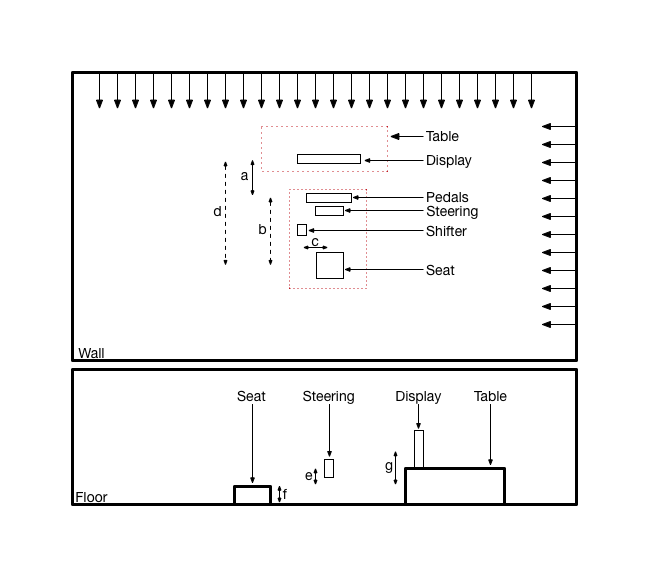
\includegraphics[width=\textwidth]{images/experiment-setup-schematic.png}
	\caption[Experiment Setup Schematic]{Top-down and side views of experiment setup}
	\label{fig:meth-experiment-setup}
\end{figure}

%Feedback to participants could have been provided mainly in two ways, visually through a heads up display or auditory by means of descriptive speech. During initial prototypes for the feedback system, feedback was conveyed using a heads up display approach, however this proved to be too distracting for users, furthermore there where issues trying to provide meaningful feedback by means
%of text or pictures on screen overlayed over the sim game. Users found the feedback hard to interpret at a glance. The heads up display was changed in favour of an auditory feedback, as it is less introduce\cite{leahy2003auditory}. It would have been interesting to look into a hybrid approach in which auditory feedback is aided with heads up display. This might have been especially beneficial in cases in which the feedback needed to convey degrees or ranges. However, due to time constraints it was settled to have a sole auditory system.
%
%\subsubsection{Track and car choice}
%The track and car choice was made based on mainly on suggestions off the study by Bastow et al, Car suspension and handling who suggest front wheel drive  cars being easier to drive. This is due to front wheel drive tend to understeer more which results in more predictable cornering, while also being less effected by sudden changes in throttle application. In comparison rear wheel drive cars tend to be less predictable in corners as being more sensitive to sudden changes to throttle application and wieght transfer resulting in oversteer which is harder to control. The track should be as flat and smooth as possible in rdetr to avoid any drastic changes to the car geometry due to an even surfaces or bumps which may result is loose of control. The track also needs to have wide run off areas. these areas are located along the circuit where racers are most likely to unintentionally depart from the prescribed course. This gives the racers time to slow down before colliding with stationary objects.

\subsection{Experiment Materials}
\label{sec:meth-experiment-setup}
The setup of the experiment was divided into three material categories: \emph{simulation environment}, \emph{simulation hardware} and \emph{simulation software}, with each category subscribing to a number of desirable properties: 

\begin{description}
	\item [Environment] The experiment should be carried out in an isolated, noise-free and well-lit room. Participants would be let in the room one at a time, to ensure the experiment is conducted without any distractions.
	\item [Hardware] The hardware components identified for this experiment are the (i) display output, (ii) steering wheel, (iii) gear shifter, (iv) acceleration, brake and clutch pedals and (v) seating frame.
	\begin{description}
		\item [Display] Xi haga fuq id-display (Make, model, resolution)
		\item [Driving Controls] The driving controls include (ii)-(iv); minimally a steering wheel should provide the same number of revolutions as a racing car, providing accurate force feedback to let the participants accurately assess the behaviour of the car. Gear shifters do not implement feedback mechanisms; however, given their ubiquity, H-shifters are preferred since they are the kind most drivers are familiar with. High-end pedal systems use hydraulics to simulate the variability of force required on part of the driver to actuate a pedal during different stages of a drive.
		\item [Seating frame] The seating frame should ensure a seating position akin to a driver in a racing car. Details re: adjustability.
	\end{description}
	\item [Software] Extract properties from commented para below:
	%The last part of the experiment setup tackles the to driving model, which has been simulated by a consumer available off the shelf sim-racing game called Assetto Corsa which is widely accepted by world wide sim racers as being a valid sim racing game which simulates the real world accurately. Assetto Corsa provides realistic car handling and characteristics vehicle models and real life racing tracks. The tracks are laser scanned, this technology manages to replicate a track surface accurately allowing this project ensure the track being used is as close as possible to the real track. In addition, Assetto Corsa also provides the fucntionality to disable any damage, wear and tear of the car, which allows for better constant variables as cars will not get progsivley worse during a session hindering a participants. Although there are other sim racing games which provide the same level of realism such as Project Cars and iRacing, Assetto Corsa has the advantage of an easy to use telemetry API which any programming language can access and a strong community of developers who can help should one need assistance on the API use.
\end{description}

To add tabulated properties for the choices considered and rationale for the final equipment/software procured.

%It was important for the experiment setup to be able to make participants feel as if they are driving a real car, yet being able to keep within the constraints of the budget which aims to use of off the shelf, consumer affordable items. Furthermore, any environment variables had to be controlled as much as possible in order to avoid any inherited bias ending favouring a particular participant.

%\subsubsection{Environment}
%Ensuring all participants were exposed to the same testing environment allowed to have any bias to be introduced. Distractions could have played a major role in a participant's performs. As such the experiments have been carried out in a closed room, free from any noise from crowds. One participant at a time was allowed in the room, this avoid having other participants gaining any information from other participants' experiments while also avoiding participants distracting each other. The room which is to be used for the experiments has two walls with windows facing the out side which in the morning has sun light come in directly, in cases potentially temporally blinding a participant during an experiment. To avoid this, the setup is placed to a location in the room in which sun rays do not effect participants during any time of the day,

%\subsubsection{Hardware}
%With hardware being the most expensive part of this research, it was important to be able to find a good balance between cost and and quality. In this case quality refers to the ability a piece of hardware has to convey the sense of realism to a participant. Starting off with the steering wheel set, it had to be able to turn as much as a race car wheel and be able to accurately replicate the forces a race car steering wheel experiences during use. This is done through force feedback technology, which allows participants to better feel what the car is doing. An H shifter and pedals were also required. Shifters don't vary much, as force feedback technology is not implemented in these devices, however it was important to use an H shifter as this is what most participants are expected to be familiar with this type. Moving on the pedals, there are sets which try to replicate varying pressure for brake and clutch pedals using hydraulic actuated pistons which is what one expects to find in a real car. These pedals set are very good and replicating the force one is required to use while braking or activating the clutch, however these are very expensive and as such fail out of budget. As such a more entry level set has been used which still performs well.
%The steering and other mentioned peripherals were attached to a home made racing rig, which was built using the seating position one would experience in a race car, this is typical a low seating position the steering wheel and shifter close to the driver. In addition a racing seat off a local race car has been fitted with the aim of giving further sense of immersion to participants by using and replicating properties a race driver experiences.\\
%With virtual reality being introduced in recent years and gaining traction, it was looked at as a possibility as means to integrate it into the system. During initial testing virtual reality was proving to an important component, helping users get completed immersed into the simulator. However, users were getting dizzy and some had eye irritation as a result virtual reality had to be abounded.
%
%<Insert comparison chart here and say something about it>

%\subsubsection{Software}
%The last part of the experiment setup tackles the to driving model, which has been simulated by a consumer available off the shelf sim-racing game called Assetto Corsa which is widely accepted by world wide sim racers as being a valid sim racing game which simulates the real world accurately. Assetto Corsa provides realistic car handling and characteristics vehicle models and real life racing tracks. The tracks are laser scanned, this technology manages to replicate a track surface accurately allowing this project ensure the track being used is as close as possible to the real track. In addition, Assetto Corsa also provides the fucntionality to disable any damage, wear and tear of the car, which allows for better constant variables as cars will not get progsivley worse during a session hindering a participants. Although there are other sim racing games which provide the same level of realism such as Project Cars and iRacing, Assetto Corsa has the advantage of an easy to use telemetry API which any programming language can access and a strong community of developers who can help should one need assistance on the API use.

\subsubsection{Questionnaire}
Questionnaires allow for further insight from the point of view of the participants. Leary et al. provide seven guidelines for compiling a questionnaire \cite{leary}:
\begin{enumerate}
	\item being specific and precise in phrasing the questions
	\item writing the questions as simply as possible, avoiding difficult words, unnecessary jargon, and cumbersome phrases
	\item avoid making unwarranted assumptions about the respondents
	\item conditional information should precede the key idea of the question
	\item do not use double-barrelled questions
	\item pretest the questions
\end{enumerate}
%(i) being specific and precise in phrasing the questions, (ii) writing the questions as simply as possible, avoiding difficult words, unnecessary jargon, and cumbersome phrases, (iii) avoid making unwarranted assumptions about the Respondents, (iv) conditional information should precede the key idea of the question, (v) do not use double-barreled questions, (vi) choose an appropriate response format and (vii) pretest the questions. 
Responses from questionnaires designed using these guidelines are valid in the general case. The challenge in choosing a response format in a question lies in identifying whether one should go for an open ended question in which more information might be collected, or on the other hand, use a rating scale response format, where the response is more constrained but may be easier to analyse. Leary et al. suggest using the former for questions dealing with behaviours, thoughts, or feelings that can vary in frequency or intensity (e.g. the Likert Scale\cite{likert1932technique}) and using open ended questions in cases where further insight is desired.

Based on these guidelines two qualitative questionnaires have been designed, one aiming to gather insight into the sample demographic, the other aiming to gain insight into the participants' impressions about the realism of the experiment setup, the level of comfort, or discomfort and any suggestions or comments they might have. 

\subsection{Procedure}
\label{sec:meth-experiment-structure}
In order to evaluate the effectiveness of the system a user study took place. Participants were split randomly into two groups. One group will be referred as the feedback group, the other will be referred to as the base group. The experiments structure was subdivided into smaller systemic tasks.

\begin{description}
	\item[Demographic questionare] At the start on the experiment the demographic questionare is to be handed out to the participant.
	
	\item[Adjust Rig Configuration] In order for the participant to sit comfortable while also ensuring all controls can be reached with ease, the rig has to be configured per participant. This involves having to move the seat further back or forward to the steering wheel, as it would be done in a real car. In addition participants are also told how to operating the rig. The explanation covers the steering wheel turns two and a half turns from lock to lock, the pedals are setup as on any manual road car, having the clutch pedal on the left, brake in the middle, and throttle on the right. The H shifter is also explained by having a run through demonstration of all gears which allows participants to be able to operate the rig with out having to learn on their own.
	
	\item[Breaks] To avoid having driving sessions possibly put too much strain on participants, optional five minute breaks are allowed to be taken between driving sessions. 
	
	\item[Ten minuties practice] During these ten minutes users are told to simply get used to the rig setup, track and car. The aim of this session is for participants to get used to the setup while also allow this study to measure their skill before the feedbvack system as the independent variable is introduced.
	
	\item[Two Ten minuties sessions] These are the sessions in which the feedback system is turned on for the feedback group, while the participants in base group are left to keep trying to improve without any aid. 
	
	\item[Five minuties session] A final five minuties of driving are allocated yet again, this time with the feedback system turned of for both groups. This was designed to possibly identify any conclusive results. Such session could show the possibility of the feedback group performing worst after having the aid of the feedback system removed or both groups ending up perofmring the system after the sessions suggesting the feedback participant didn't manage to get any cognitive advantage.
	
	\item[Particpant's feedback questionare] The final stage of the experiment requires participants to fill in the a questionnaire  in which they are asked to give their feedback on the experiment structure, hardware used and any further comments they would like to add.
	
\end{description}

\subsection{Data Collection and Sampling}
\label{sec:meth-data-gathering}
At the end of the experiments the data collected includes two questioners from each participant and four batches of telemetry data, one for each participant. Questioners are filled online using Google Forms as it provides the ability to export the data and also automatic generation of descriptive statistic in conjunction with representing the results via data visualisation techniques such as bar charts and pie charts. The data collected from the questionnaires and telemetry data is to be loaded into a data base management system from which the data can be queried using specialised data querying constructs. This is done as the telemetry data collected contains around 200,000 records per participant, which proved to be too much to handle at once during analysis. By having a querying language, it provides the flexibility of extract data which is relevant for the data analysis at hand.

\subsection{Data Analysis}
\label{sec:meth-data-analysis}
In order to accept or reject the null hypothesis tests for mean scores on two independent groups. By carrying out this test one is able to determine to a level of confidence the effect caused by the introduction of the independent variable, which in this case refers to the feedback system. The lap time is used as the test variable as this gives a good indication for the average performance achieved during a lap. 

https://statistics.laerd.com/spss-tutorials/mann-whitney-u-test-using-spss-statistics.php
For dataset small than 2000 elements, we use the Shapiro-Wilk test, otherwise, the Kolmogorov-Smirnov test is used. In our case, since we have only 20 elements, the Shapiro-Wilk test is used
Normality tests are to be carried out to determine the distribution. After which it will be possible to use Independent samples t-test\cite{siegel1956nonparametric} as 
the distribution was normally distributed, from such test one can determine the degree of influence in the introduction of a variable has had over a group. In case the data is not normally distributed the non parametric Mann Whitney test as there is no need to assume a normal distribution.